\usetikzlibrary{calc}
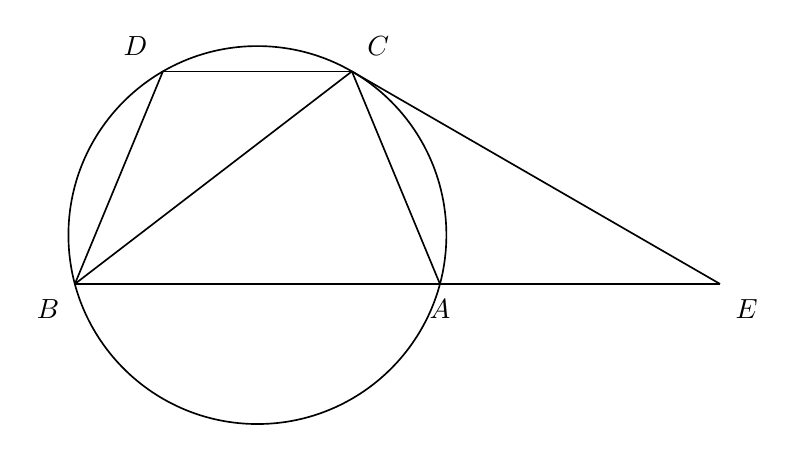
\begin{tikzpicture}[x=1cm,y=1cm,line width=.6pt,font=\normalsize]
\coordinate (O) at (0,0);
\coordinate (D) at (-1.2,2.0785);
\coordinate (C) at (1.2,2.0785);
\coordinate (B) at (-2.3182,-0.6212);
\coordinate (A) at (2.3182,-0.6212);
\coordinate (E) at (5.8759,-0.6212);
\draw (O) circle[radius=2.4cm];
\draw (D)--(C);
\draw (D)--(B);
\draw (B)--(C);
\draw (C)--(A);
\draw (B)--(E);
\draw (C)--(E);
\node[above left=2pt] at (D) {$D$};
\node[above right=2pt] at (C) {$C$};
\node[below left=2pt] at (B) {$B$};
\node[below=2pt] at (A) {$A$};
\node[below right=2pt] at (E) {$E$};
\end{tikzpicture}
